\section{Metodología}
    El primer paso a realizar en esta investigación es recrear el código de John Bullinaria,
    para esto se va a utilizar el repositorio de Optical Digits, al momento de obtenjer estos datos
    ya se va a poder comenzar con la programación en Python.

    Al momento de comprobar que el código funciona como el algoritmo de John, se realizarán modificaciones
    que permitirán repartir las tazas de aprendízaje con estos valores.

    Para obtenerlo se usarán metodologás como el Backpropagation y funciones de activación tal como la Sigmoidal.

    Cuando los dos proyectos se tengan, se realizara una comparación, donde se vera cual de estos dos experimentos
    es más eficaz en proyectos de la vida real.
    
\section{Cronograma de Actividades}

    \begin{figure}[H]
        \centering
        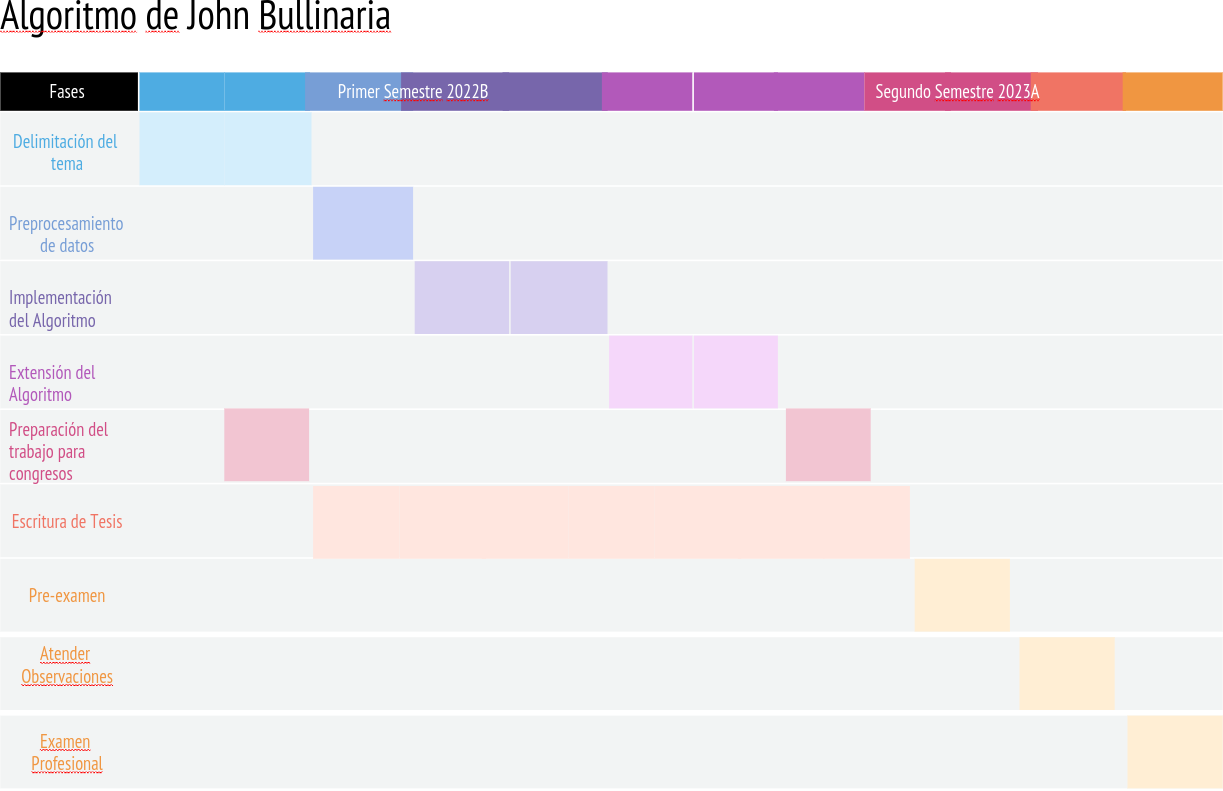
\includegraphics[width=\columnwidth]{diagramaGantt.png}
        \caption{Diagrama de Gantt}
        \label{fig:fig3}
    \end{figure}

\section{Organización del Capitulado}